\documentclass[a4paper,11pt]{ltjsarticle}
% 数式
\usepackage{amsmath,amsfonts}
\usepackage{bm}
% 画像
\usepackage{graphicx}
\usepackage{circuitikz}
\usepackage{amsmath,amssymb}
\usepackage{siunitx}
\usepackage{float}
\usepackage{tikz}
\usepackage{askmaps}
\usepackage{multirow}
\usepackage{bigstrut}
\usepackage{slashbox}
\usepackage{rotating}
\usepackage{listings}
% 数式
\usepackage{physics}
\usepackage{mathtools}
% 画像
\usepackage{subcaption}
% 表
\usepackage{makecell}
% その他
\usepackage{url}
\usepackage{ascmac}
\usepackage{cases}
\usepackage{here}
\usepackage{upgreek}
% 日本語対応
\usepackage{luatexja}
\usepackage{luatexja-fontspec}

\AtBeginDocument{\RenewCommandCopy\qty\SI}


\definecolor{commentgreen}{RGB}{0,200,0}
\definecolor{eminence}{RGB}{120,80,250}
\definecolor{weborange}{RGB}{255,165,0}
\definecolor{frenchplum}{RGB}{10,150,200}
\definecolor{commentgreen}{RGB}{0,200,0}
\definecolor{eminence}{RGB}{120,80,250}
\definecolor{weborange}{RGB}{255,165,0}
\definecolor{frenchplum}{RGB}{10,150,200}

\lstset{
        language = {C},
        basicstyle = \ttfamily\small,
        keywordstyle=\color{eminence}\ttfamily\bfseries,
        commentstyle=\color{commentgreen}\textit,
    identifierstyle=\color{black}\ttfamily,
        xleftmargin=.35in,
        frame=lines,
    showstringspaces=false,
        numbers=left,
        stepnumber = 1,
        breaklines=true,
        numberstyle = \ttfamily\normalsize,
    tabsize=4,  
        emph={int, int8_t, int16_t, int32_t, int64_t, uint8_t, uint16_t, uint32_t, uint64_t, char, double, float, unsigned, void, bool},
        emphstyle={\color{blue}}, 
        morekeywords={>, <, ., ;, +, -, *, /, !, =, ~},
        breakindent = 10pt, 
        framexleftmargin=10mm, 
        columns=fixed,
        basewidth=0.5em,
        }

% 特定のスタイル設定
\lstdefinestyle{customtxt}{
  basicstyle=\ttfamily\footnotesize,
  backgroundcolor=\color{lightgray},
  frame=single,
  breaklines=true,
  columns=fullflexible,
  showspaces=false,
  showstringspaces=false,
  showtabs=false,
  tabsize=4,
}

\newcommand{\fig}[4]{
    \begin{figure}[htbp]
      \centering
      \includegraphics{./images/#1}
      \caption{#2}
      \label{fig:#3}
    \end{figure}
  }
\begin{document}
\begin{flushright}
    22060 古城 隆人\\
\end{flushright}

\section{実験結果}
二分法,はさみうち法,ニュートンラプソン法において,式\eqref{eq:func}の解を
Excelを用いて求めた.
\begin{equation}
    f(x) = \cosh(x)\cos(x) + 1
    \label{eq:func}
\end{equation}
各方式の初期条件を表\ref{tab:init}に示す.
この初期条件を持ちて,xと解の関係をグラフ\ref{fig:result}に示す.
\begin{table}[H]
    \centering
    \caption{各方式の初期条件}
    \begin{tabular}{|c|c|c|}
        \hline
        方式         & 初期値1 & 初期値2 \\ \hline
        二分法        & 0    & 2    \\ \hline
        はさみうち法     & 0    & 2    \\ \hline
        ニュートンラプソン法 & 2    & -    \\ \hline
    \end{tabular}
    \label{tab:init}
\end{table}
\begin{figure}[H]
    \centering
    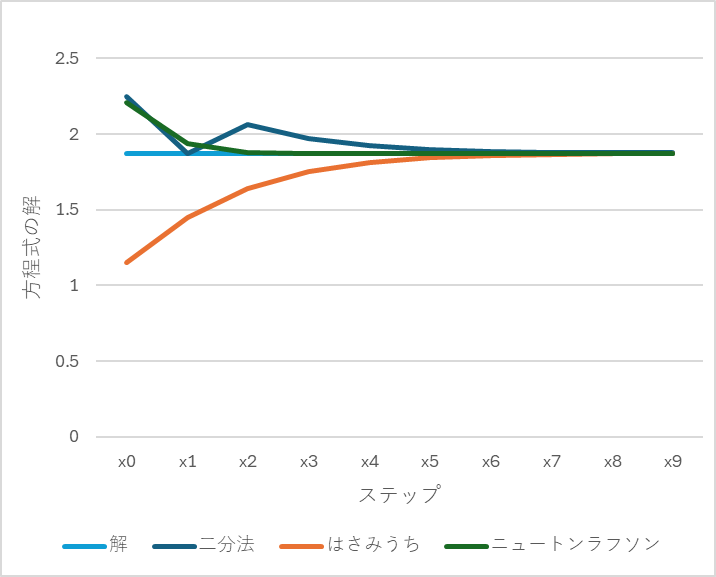
\includegraphics[width=12cm]{./images/result.png}
    \caption{各方式の結果}
    \label{fig:result}
\end{figure}




\end{document}